\begin{frame}

  \frametitle{Logique combinatoire}
  \framesubtitle{Portes logiques}

  \begin{figure}

    \centering
    \includegraphics[width=\linewidth]{figs/gates.pdf}
  \end{figure}

\end{frame}


\begin{frame}

  \frametitle{Logique combinatoire}
  \framesubtitle{Binaire}

  \begin{center}
    \begin{tabular}{ |c|c||c|c||c|c| }
     \hline
     A & B & $\Sigma$ & C & $A\oplus B$ & $A\land B$  \\
     \hline
     0 & 0 & 0 & 0 & 0 & 0\\
     \hline
     0 & 1 & 1 & 0 & 1 & 0\\
     \hline
     1 & 0 & 1 & 0 & 1 & 0\\
     \hline
     1 & 1 & 0 & 1 & 0 & 1\\
     \hline
    \end{tabular}
  \end{center}


  \begin{figure}

    \centering
    \includegraphics[width=0.4\linewidth]{figs/adder.pdf}
  \end{figure}


\end{frame}


\begin{frame}

  \frametitle{Logique combinatoire}
  \framesubtitle{Implémentation}

  \begin{figure}

    \centering
    \includegraphics[width=\linewidth]{figs/elecDiag.pdf}

  \end{figure}


\end{frame}


\begin{frame}

  \frametitle{Logique combinatoire}
  \framesubtitle{Implémentation}



  \begin{figure}

    \centering
    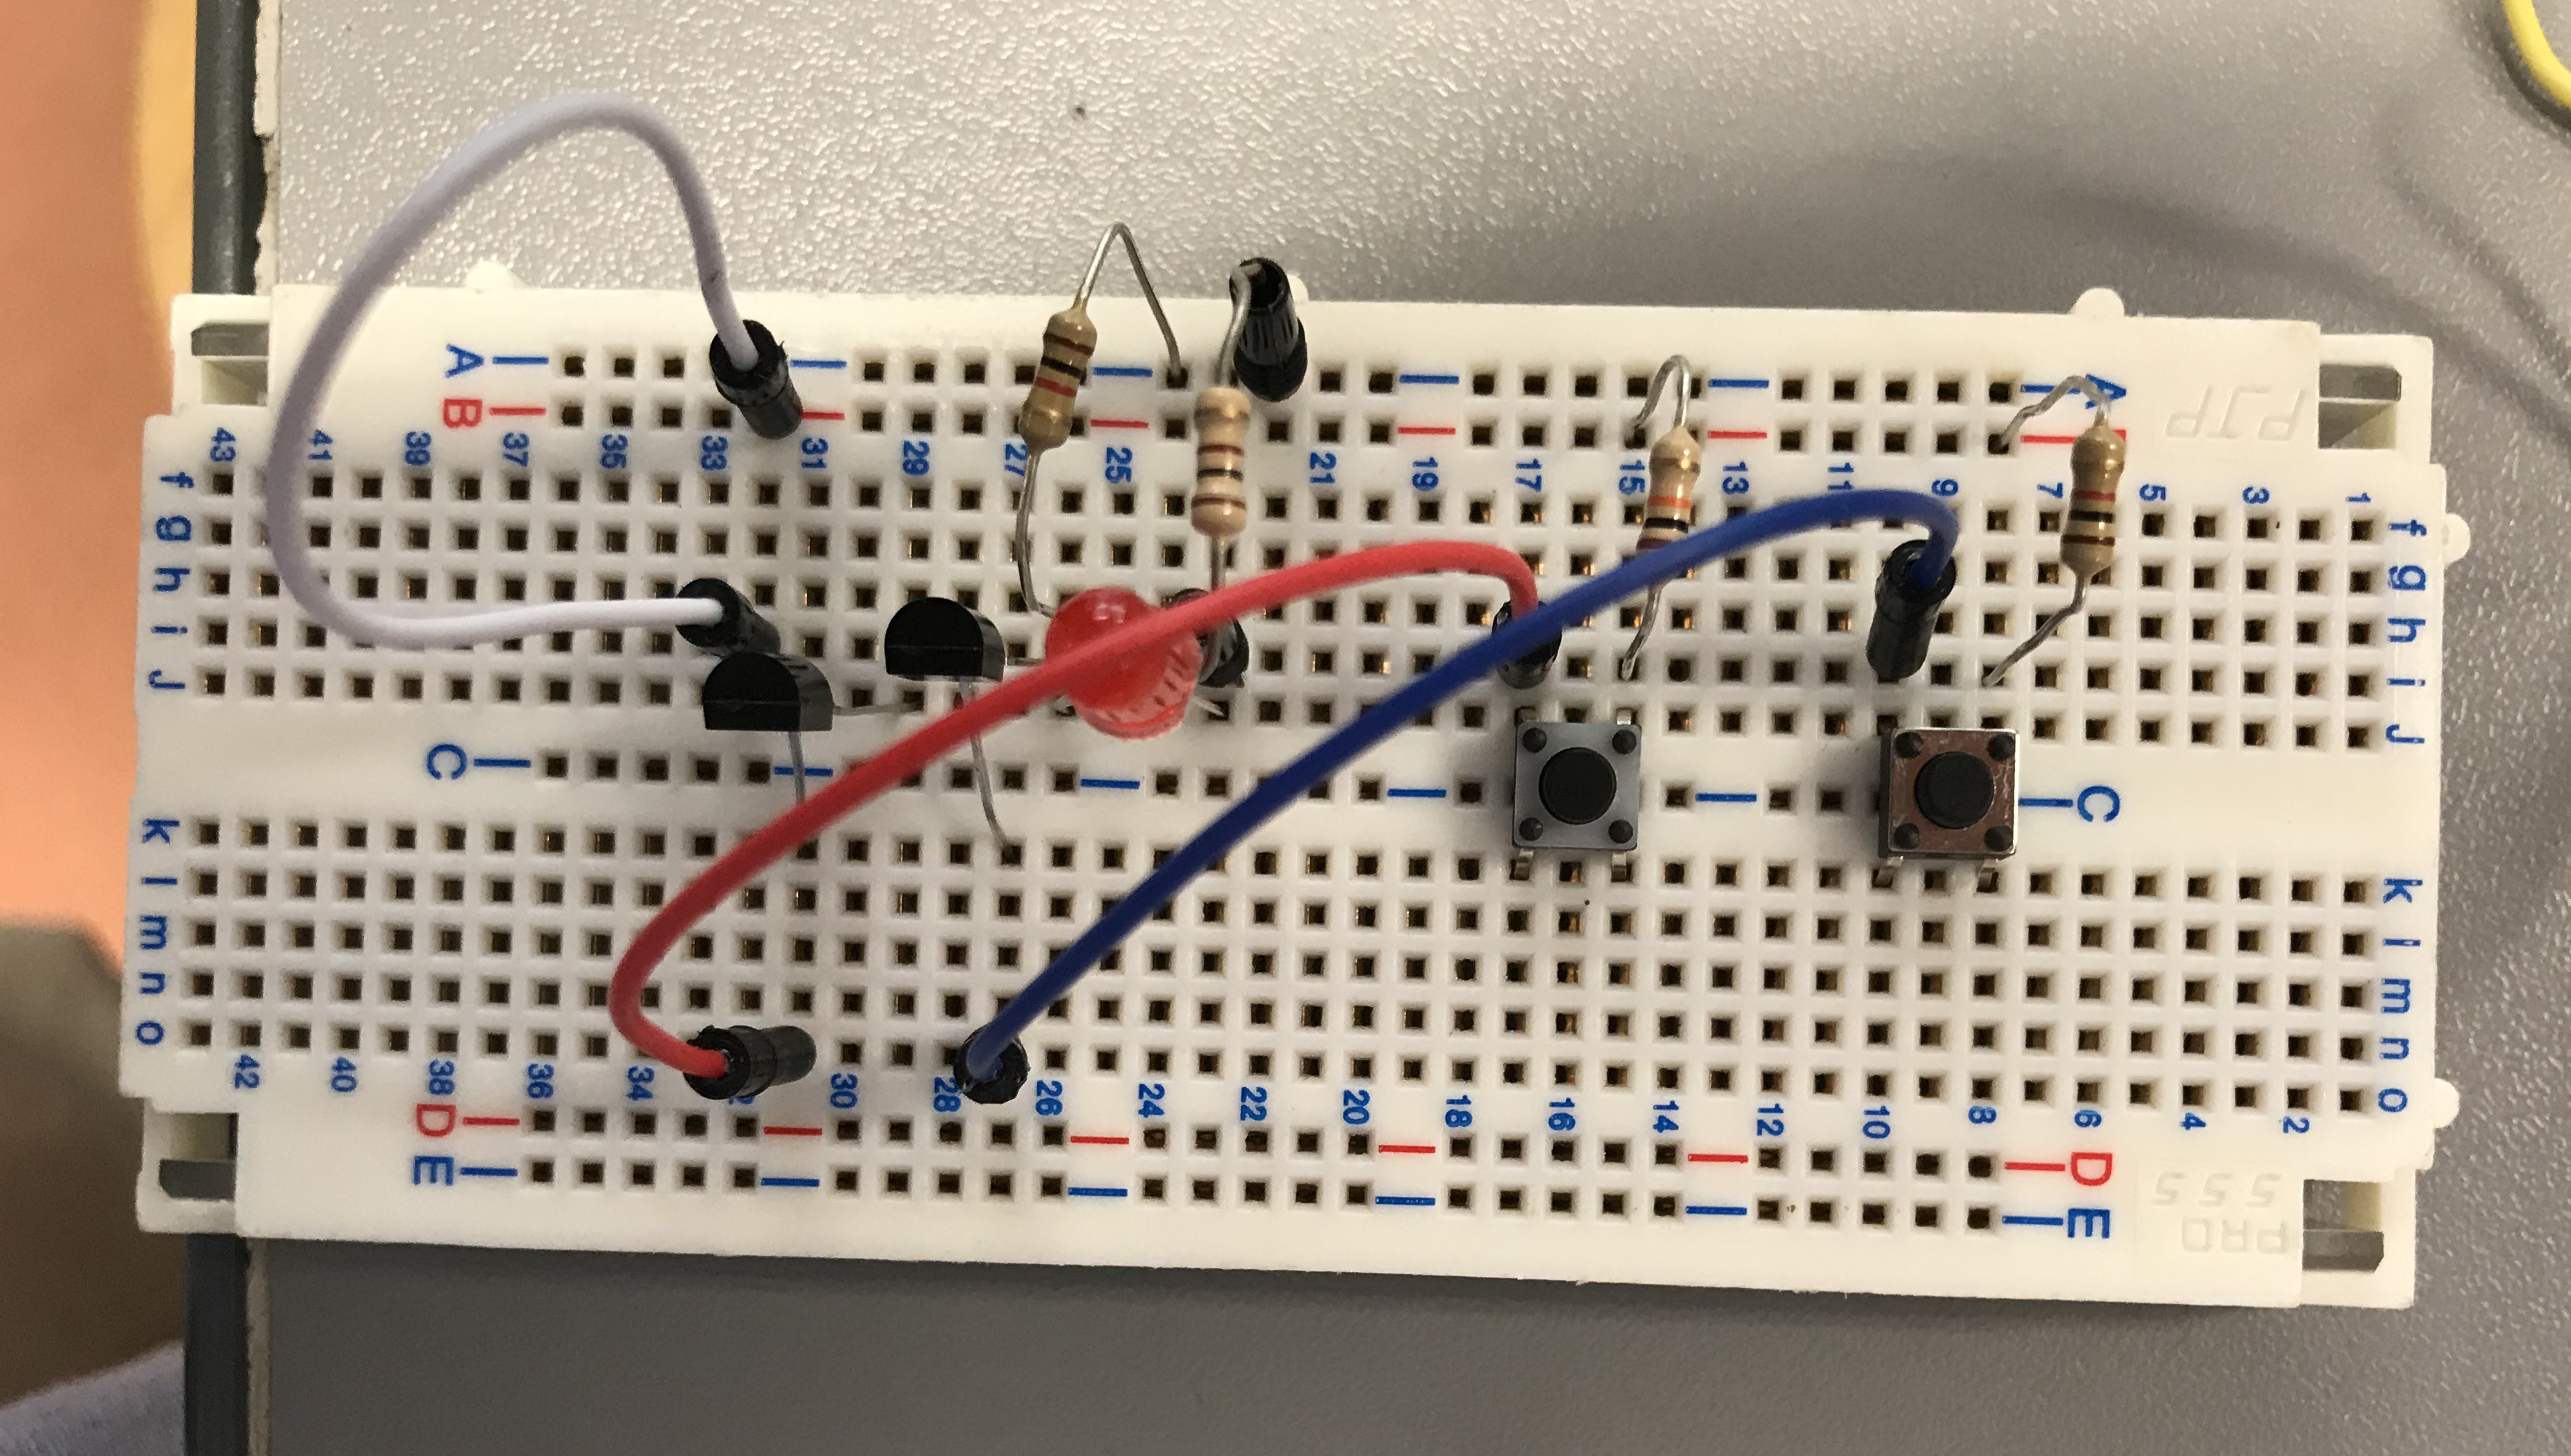
\includegraphics[width=\linewidth]{pics/and.jpg}
  \end{figure}


\end{frame}
